\documentclass[11pt]{article}
\usepackage{xcolor}

\author{Computing Workshop}
\title{Friday planning}
\date{}

\usepackage{tikz}
\usepackage{listings}
\usepackage[margin=2.0cm]{geometry}
\usetikzlibrary{arrows}

\lstset{
  basicstyle=\ttfamily
}

\begin{document}

\maketitle

To minimize decision paralysis, we're going to create an algorithm that tells us what to do on a Friday based on a
number of inputs. First we must collect data. Enter in the two most common things you do on a Friday night, which
we'll assume are the only things you do Fridays.
\begin{enumerate}
  \item
    \color{gray}{\emph{Ex. going out with friends}}
  \item
    \color{gray}{\emph{Staying in and study}}
\end{enumerate}

In the name of making an accuracte algorithm, reflect on 3 things that influence what you decide to do on a Friday night.

\begin{enumerate}
\item
  \color{gray}{\emph{Ex. Amount of tests coming up}}

\item

  \color{gray}{\emph{Nice weather outside}}
\item

  \color{gray}{\emph{All your friends are going out}}
\end{enumerate}

In order to make an accurate predictor, we need to know which reasons have a push or pull effect on what you'll do for
that night. For example, nice weather might make it more likely you'll go out,
but all your friends going out might have and even stronger
weight to it. Fill in the table to weigh your reasons, indicating whether you are more or less inclined to going
and by how much, a lot, little, or no change.

\begin{center}
  \renewcommand{\arraystretch}{2.0}
\begin{tabular}{| p{14em} | p{14em} | p{14em} |}
    \hline % Use hline to make horizontal lines between rows
    \textbf{Reason} & \textbf{Influence on first option} & \textbf{Influence on second option} \\ \hline
    \color{gray}{\emph{All your friends are going out}} & \color{gray}{\emph{more inclined by a lot}} & \color{gray}{\emph{less inclined by a little}} \\ \hline
    ~ & ~ & ~ \\ \hline
    ~ & ~ & ~ \\ \hline
    ~ & ~ & ~ \\ \hline
\end{tabular}
\end{center}

Now that we have the appropriate data, let's use a neural network framework to create a decision making algorithm. The
first step is drawing out the reasons and options out in a graph, with the first column of nodes will be the influencing
reasons, and the next column of nodes will be the options for your Friday night.


\begin{figure}[h]
  \centering
  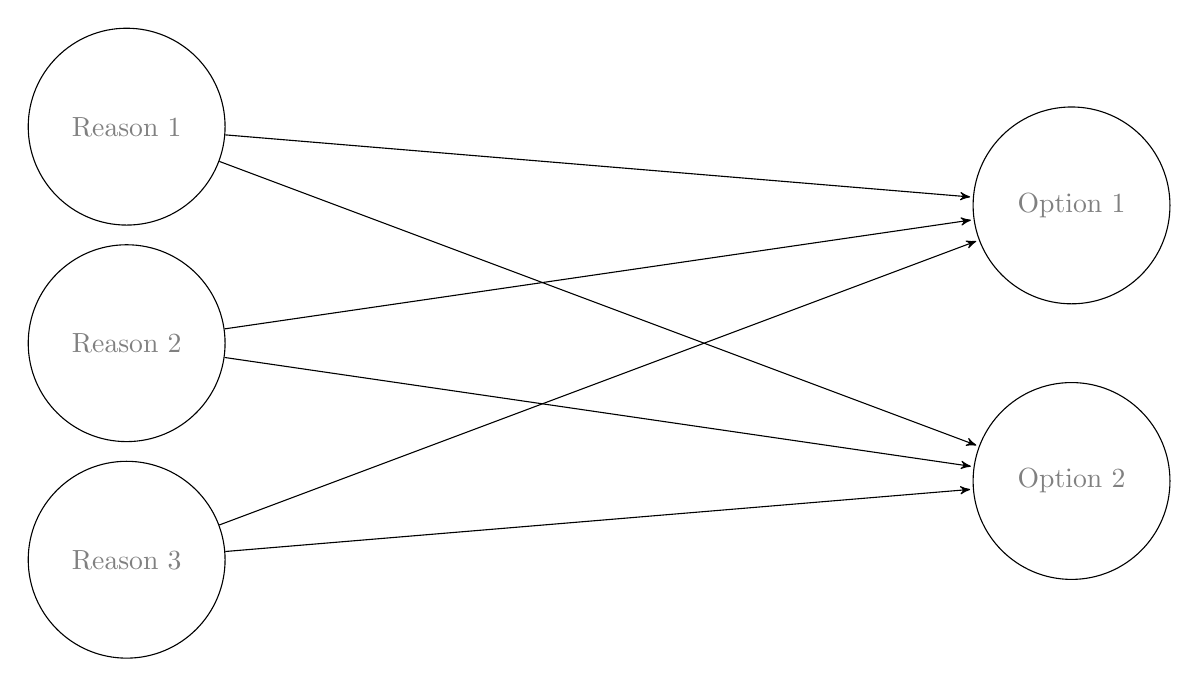
\begin{tikzpicture}[->, >=stealth', minimum size=2.5cm, shorten >=1pt]
    \node[draw, circle] at (-6, 2.75) (input1) {\textcolor{gray}{Reason 1}};

    \node[draw, circle] at (-6, 0) (input2) {\textcolor{gray}{Reason 2}};
    \node[draw, circle] at (-6, -2.75) (input3) {\textcolor{gray}{Reason 3}};

    \node[draw, circle] at (6, 1.75) (output1) {\textcolor{gray}{Option 1}};
    \node[draw, circle] at (6, -1.75) (output2) {\textcolor{gray}{Option 2}};

    \draw (input1) -- (output1);
    \draw (input1) -- (output2);
    \draw (input2) -- (output1);
    \draw (input2) -- (output2);
    \draw (input3) -- (output1);
    \draw (input3) -- (output2);
  \end{tikzpicture}
\end{figure}

Now that we have our network drawn out, it's time to give a numeric value to our weights from before. On the line that
connects a reason to a potential plan to go out, translate the influence of that reason on a potential Friday night from
words to numbers. Ex, if all my friends going out makes me a lot more inclined that I will go out too, I might give the
weight connecting the reason to the plan as a 3 or 4.

The final step is accounting for our \emph{bias}. We all have a little bias, and that includes what we'll do on a Friday
night. We're going to add that bias directly to each node in the column for plans to go out. For example, regardless of
any other condition, one might be more inclined to go out with friends over staying in to study. This means we'll add a
positive bias to the going out option, and maybe a negative bias to staying and studying if one doesn't enjoy that.

\section*{Using your model}

Now that you have an artificial neural network framework to help you plan your Fridays, try testing it out! The way to
test it is start with the inputs. The inputs should use the same scale to represent good or bad. For example, if the
deciding factors for my network are weather and all my friends are going out, then I should use the same scale (let's
say -5 to 5) where the -5 is most undesierable (such as bad weather or no friends are going out) and 5 is most
desierable (great weather and all my friends are out).

To compute a numeric answer, the neurons in the rightmost (output) layer:
\begin{enumerate}
  \item
    multiply the activation of each neuron in the previous layer with its
    corresponding weight;
  \item
    sum all these products;
  \item
    add the bias.
\end{enumerate}
%
We can write this as an equation, but first we need to establish some notation.
%
\begin{itemize}
  \item
    Let $a_1$ be the value of the top input node, $a_2$ be the value of the
    middle input node, and so on.
  \item
    Let $b_1$ be the bias of the top output node and $b_2$ be the bias of the
    bottom output node.
  \item
    Let $w_{11}$ be the very first weight for the edge connecting the top output
    neuron to the top input neuron, and let $w_{12}$ be the weight on the edge
    between the top output neuron and the middle input neuron, and so on.
\end{itemize}
%
\textbf{Question:} following this scheme, which edge does weight $w_{22}$ belong
to?

Finally, the value of output neuron $1$ is
\[
z_1 = b_1 + w_{11} a_1 + w_{12} a_2 + w_{13} a_3
\]

Using the equation, use the neural network model to decide whether you would
pick option 1 or option 2 on Friday. Record the values you choose for the
reasons and the calculated predictions of the model in the table below.

\begin{center}
  \newcommand{\size}{7em}
  \renewcommand{\arraystretch}{2}
  \begin{tabular}{| p{\size} | p{\size} | p{\size} | p{\size} | p{\size} |}
    \hline
    \textbf{Reason 1} & \textbf{Reason 2}
    & \textbf{Reason 3}
    & \textbf{Option 1}
    & \textbf{Option 2}
    \\ \hline
    %
    ~ & ~ & ~ & ~ & ~ \\ \hline
    ~ & ~ & ~ & ~ & ~ \\ \hline
    ~ & ~ & ~ & ~ & ~ \\ \hline
  \end{tabular}
\end{center}

\end{document}
